\section{Oversampling}

\subsection{Oversampling Data Set}
Oversampling is a technique to deal with class imbalance as introduced in \cite{bloem2020methology1}. This approach reduces class imbalance by duplicating some of the given images. The majority class is identified. The remaining classes are then "oversampled" to the same number of instances as the majority class. E.g. if the majority class has 2000 instances and the minority classes have 1300 and 1400 images, then the minority classes would get 700 and 600 additional "oversampled" instances (images). The resulting dataset is visualized in figure \ref{fig:oversampling_class_distribution}.

\begin{figure}[h]
    \centering
    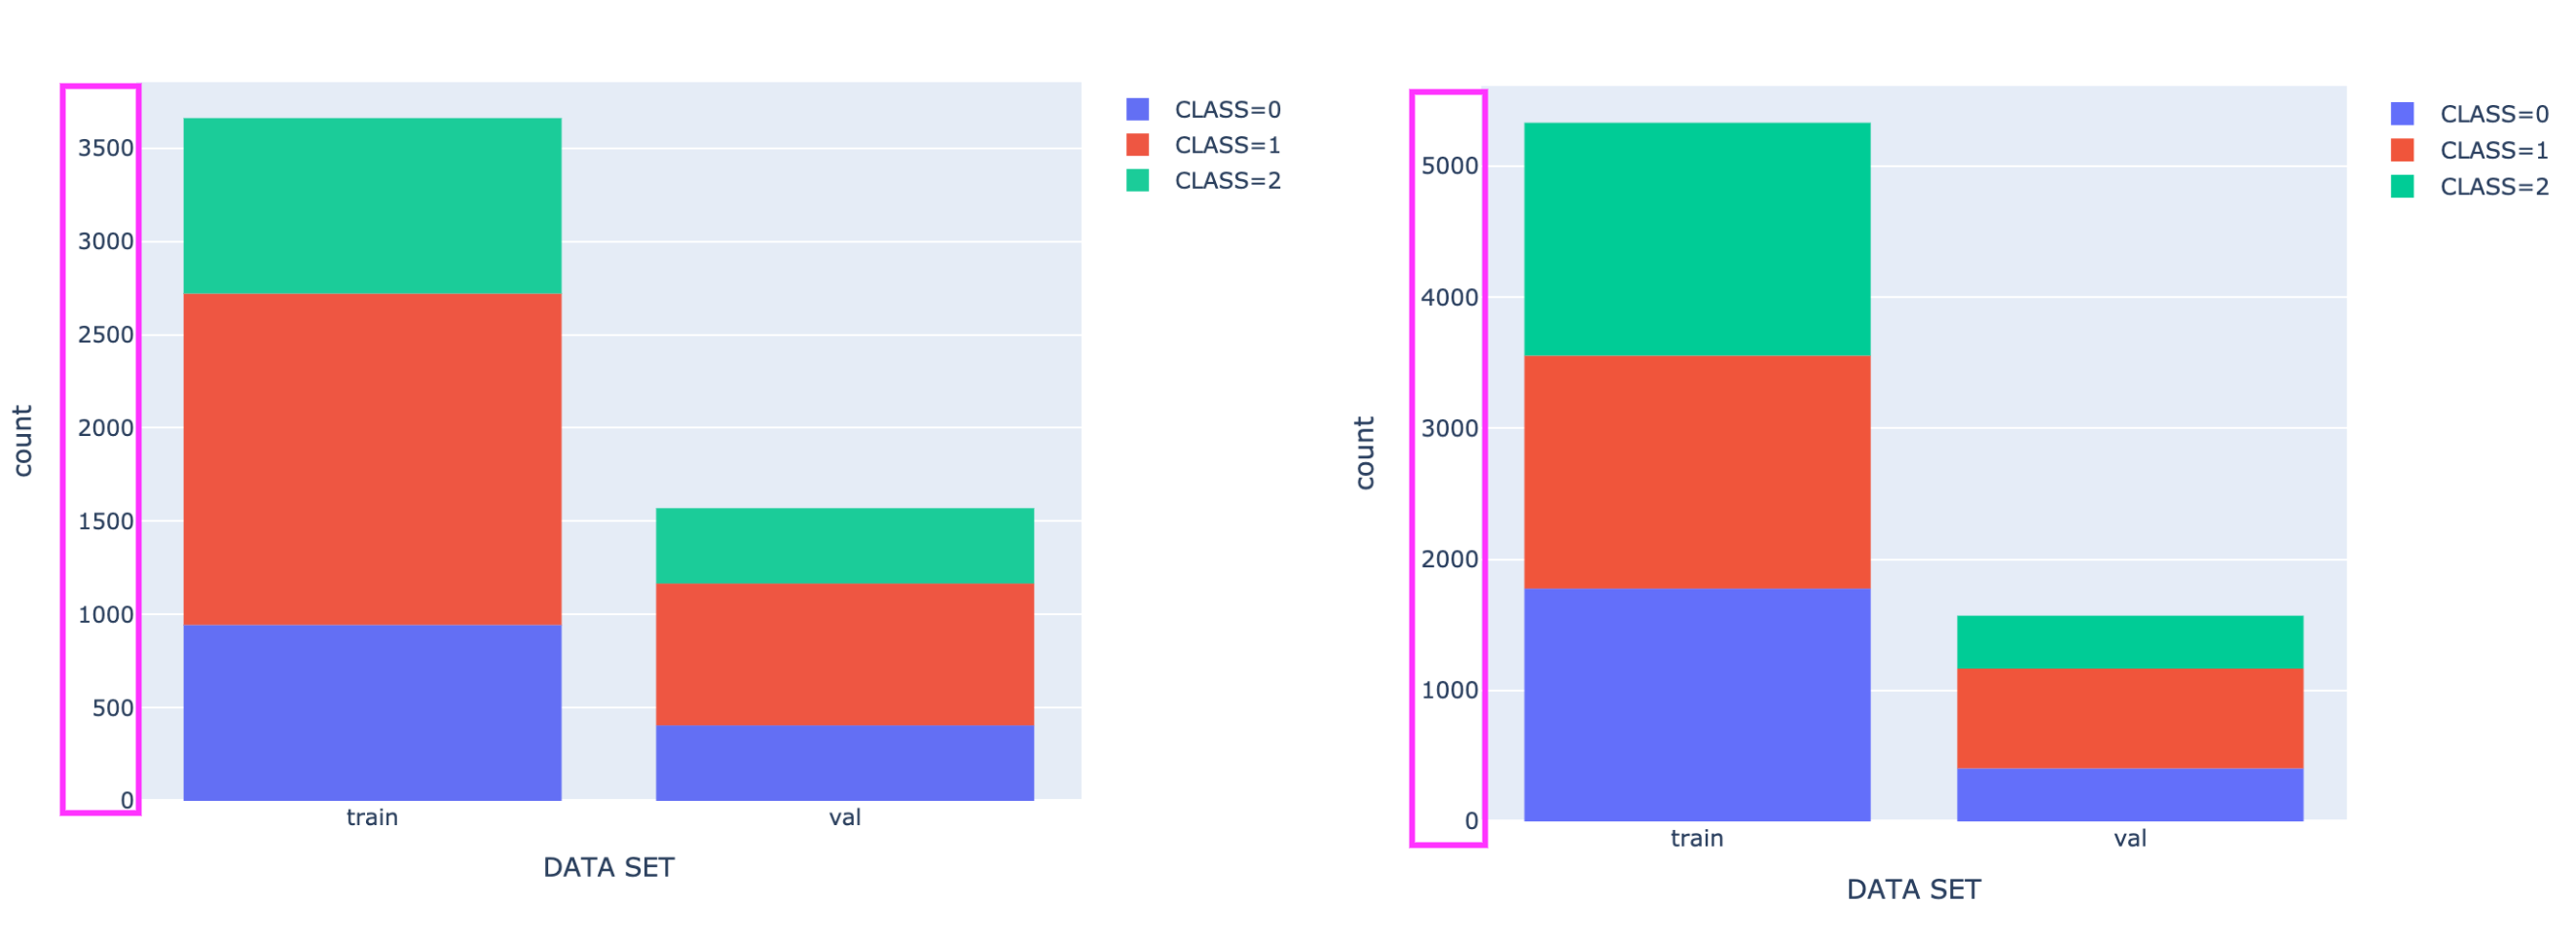
\includegraphics[width=\linewidth]{figures/oversampling/class_distribution_before_after.png}
    \caption{Class distribution after oversampling. On the left before, on the right after. Note that the y-axis is scaled to the biggest dataset. Therefore, before and after are not shown on the same scale}
    \label{fig:oversampling_class_distribution}
\end{figure}

\subsection{Results on Validation Set}
The CNN was trained three times with the oversampled data set. The results, as can be seen in the figures, show substantial worse performance in both precision and recall on the validation set compared to the baseline. While the precision on the validation set is in between a range of 0.80 to 0.82 in the baseline, the precision is only in a range of 0.27 to 0.28 using the oversampled dataset as can be seen in figure \ref{fig:over_val_a}. Likewise is the recall metric. The baselines results are in between a range of 0.78 to 0.80 while the usage of the oversampled dataset yields results in a range of 0.27 to 0.28 as can be seen in figure \ref{fig:over_val_b}.

\begin{figure}[!ht]
    \centering
    \subfloat[Precision]{\label{fig:over_val_a}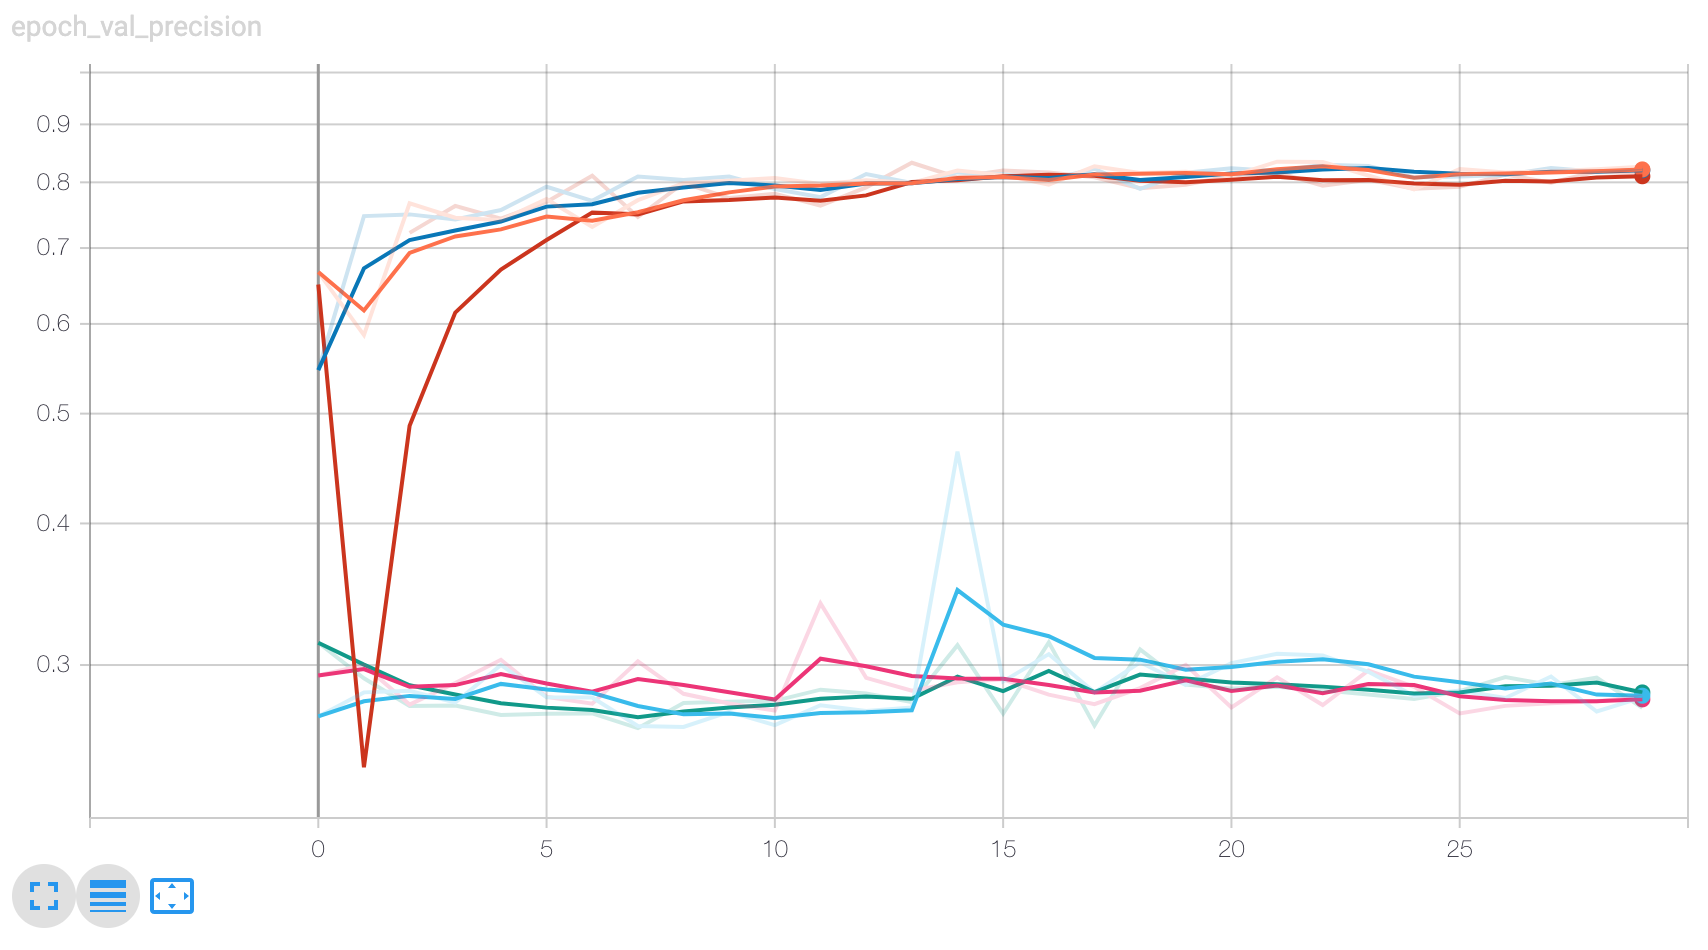
\includegraphics[width=0.89\linewidth]{figures/oversampling/val_precision.png}}
    \par\medskip
    \centering
    \subfloat[Recall]{\label{fig:over_val_b}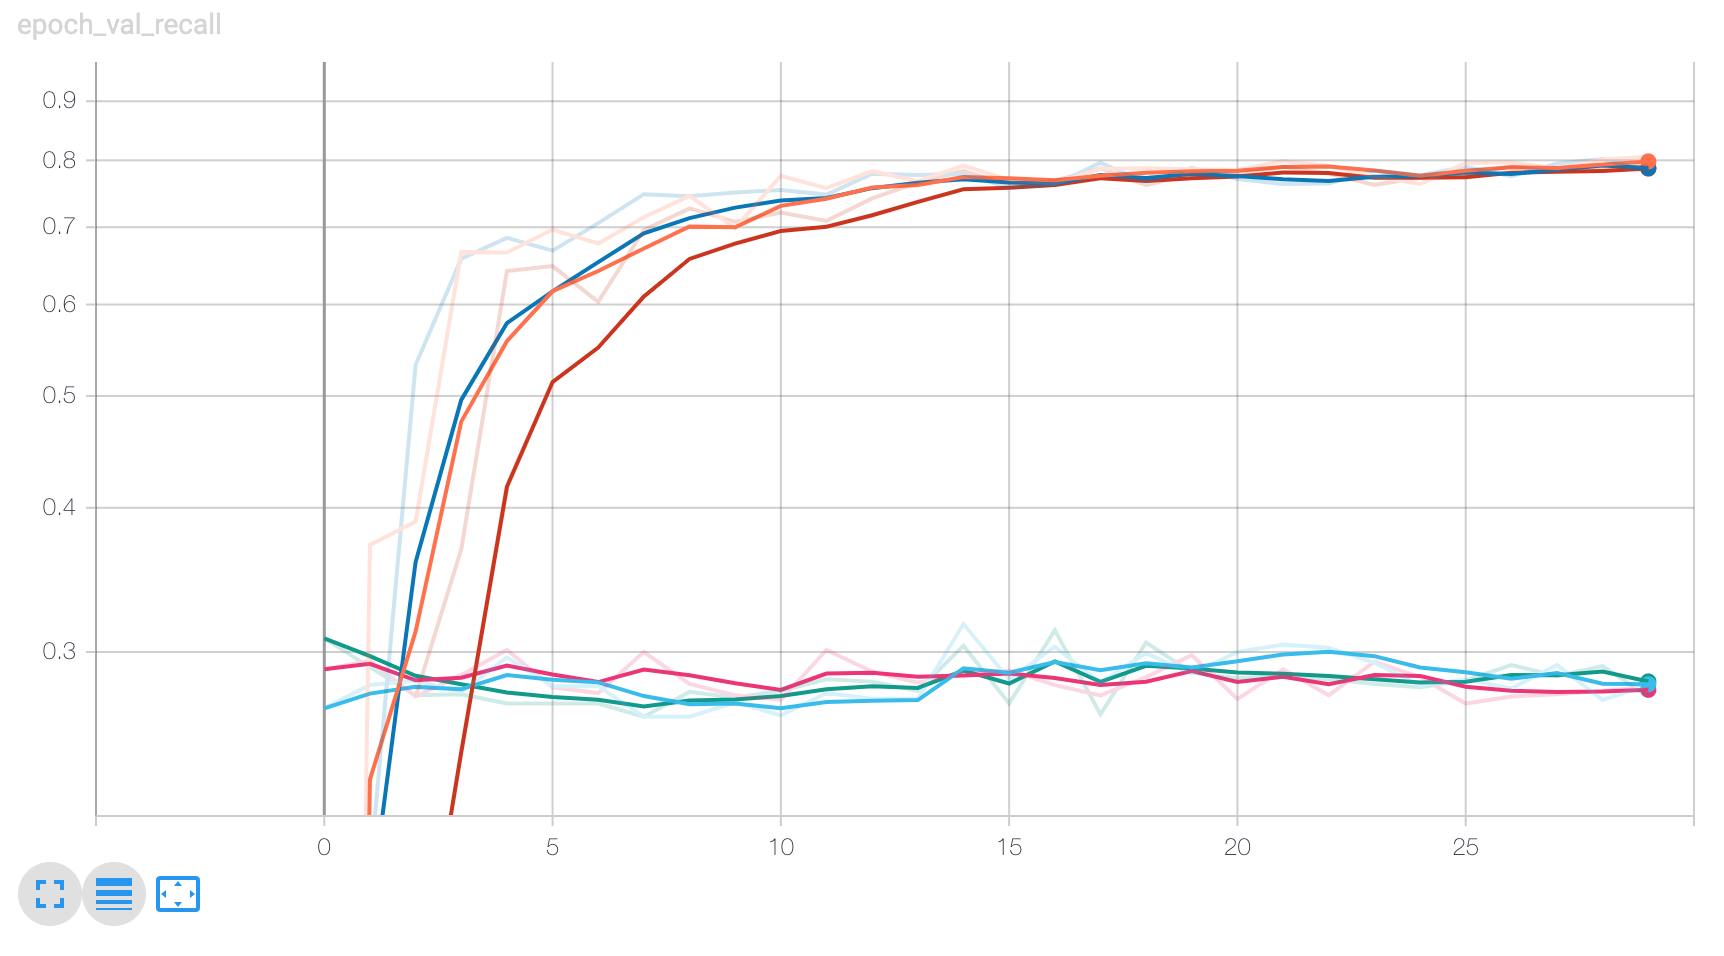
\includegraphics[width=0.89\linewidth]{figures/oversampling/val_recall.png}}
    \par\medskip
  \caption{Oversampling on Validation Set. The baselines are the three lines in the upper part of the graph. The results of oversampling are the three bottom lines. As can be seen, oversampling performs worse than the baseline.}
  \label{fig:over_val}
\end{figure}

Looking into the precision and recall results on the train set reveals that the CNN highly overfits when trained with the oversampled dataset. After already 10 batches both precision and recall above 0.995 which is near perfect when the CNN is trained with the oversampled data set as can be seen in figure \ref{fig:over_train}.
\begin{figure}[!ht]
    \centering
    \subfloat[Precision]{\label{fig:over_train_a}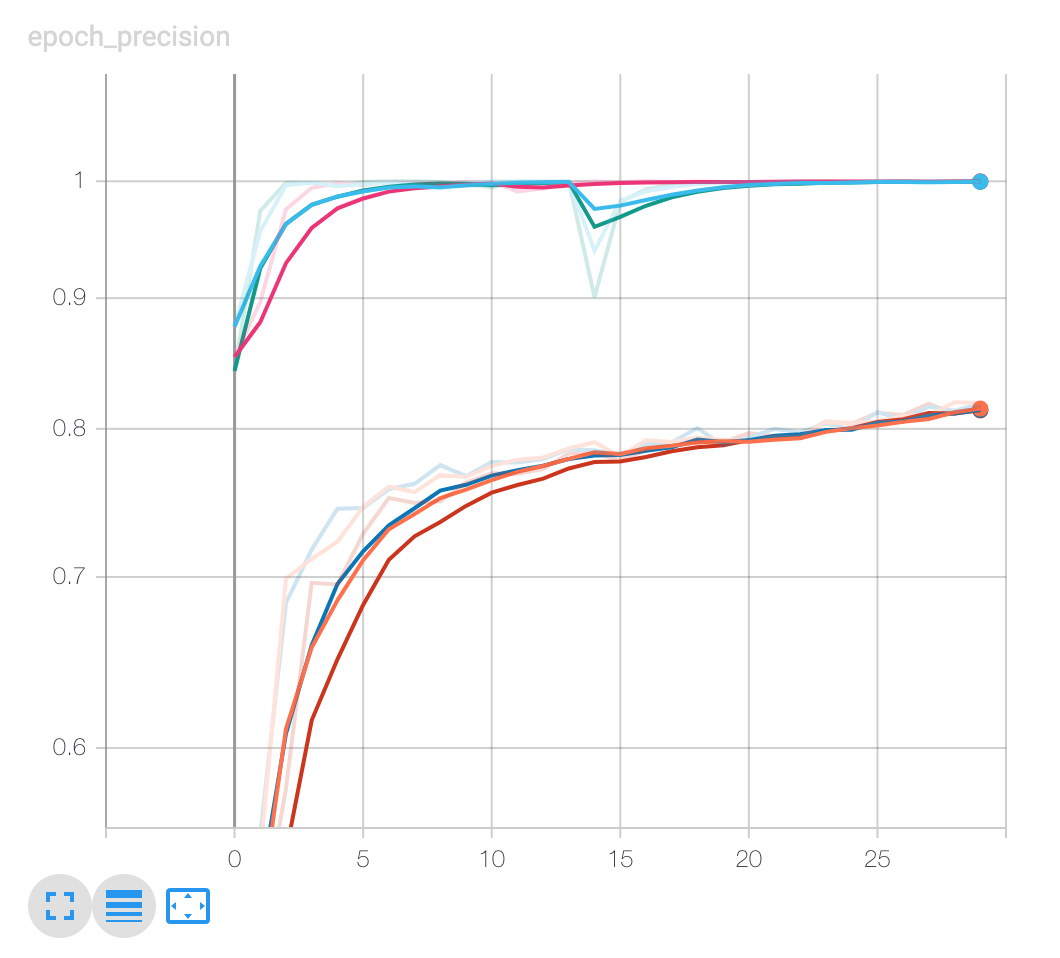
\includegraphics[width=0.89\linewidth]{figures/oversampling/train_precision.png}}
    \par\medskip
    \centering
    \subfloat[Recall]{\label{fig:over_train_b}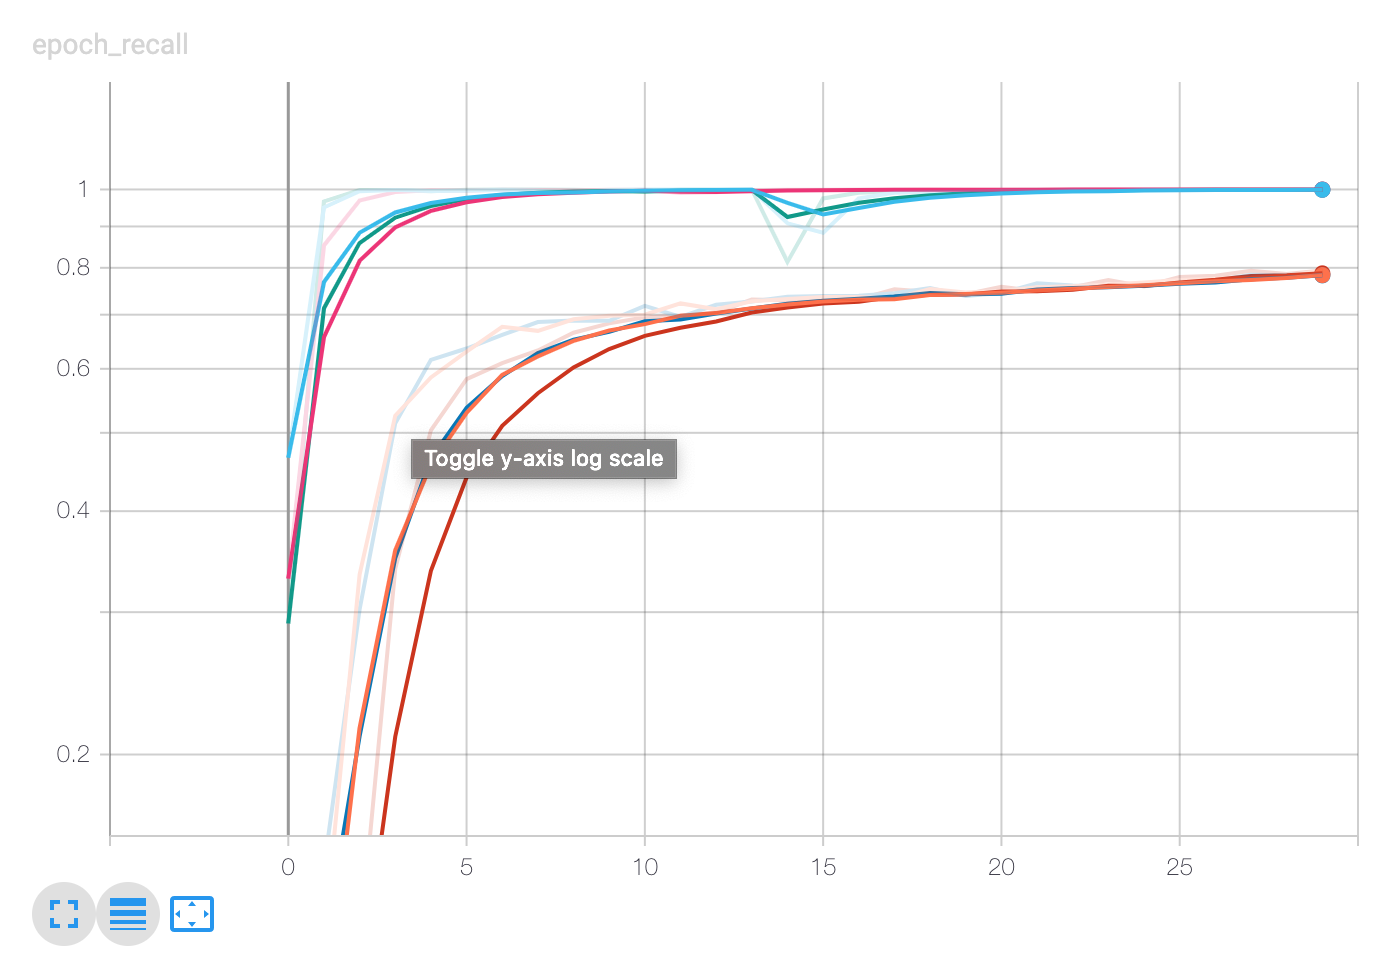
\includegraphics[width=0.89\linewidth]{figures/oversampling/train_recall.png}}
    \par\medskip  \caption{Oversampling on Training Set. The baselines are the three lines in the lower part of the graph. The results of oversampling are the three lines in the upper part of the graph. As can be seen, the oversampling results achieve near full precision and recall after a few number of batches. This implies high overfitting.}
  \label{fig:over_train}
\end{figure}

% RUN ON TEST SET

\subsection{Results on Test Set}

\begin{equation}
Precision = 0.3720
\end{equation}
\begin{equation}
Recall = 0.3702
\end{equation}

The results from on the validation set are replicated on the test set although the results on the test set are substantially higher, from around 0.27 in both metrics to around 0.37, but still way below the baseline. \\
The conclusion is drawn that oversampling in this setup leads to overfitting and therefore to worse performance. 
